\documentclass[22pt]{beamer}
\usepackage[orientation=portrait, size=custom, width=91.44, height=60,scale=1.2]{beamerposter} % 36in*2.5 = 90cm
\usepackage[absolute,overlay]{textpos}
\usepackage{bookmark} %pdflatex says to use this to avoid errors...
\usepackage{graphicx} %for including images
\graphicspath{{figs/}} %location of images
\usepackage{wrapfig} %wrap text around the images
\usepackage{listingsutf8}    %package for code environment; use this instead of verbatim to get automatic line break; use this instead of listings to get (•)
\usepackage{amsmath}
\usepackage{gensymb}
\usepackage[export]{adjustbox}
\usepackage[skins,theorems]{tcolorbox}
\usepackage{pgfplots}
\usepackage{tikz}
\usetikzlibrary{datavisualization}
\usetikzlibrary{datavisualization.formats.functions}
\usetikzlibrary{backgrounds}
\newcommand*\circled[1]{\tikz[baseline=(char.base)]{
            \node[shape=circle,draw,inner sep=2pt] (char) {#1};}}
\usepackage{array}
\usepackage{booktabs,adjustbox}
\usepackage{caption}
\captionsetup[figure]{font=scriptsize, labelfont=scriptsize}
\usepackage{ragged2e}
\usepackage{xcolor}

%\mode<presentation>
%this doesn't seem to make any difference; leave for now for trying out
\usetheme{Berlin}
\definecolor{MacBlue}{rgb}{0.10196,0.22353,0.53725}
\definecolor{MacMaroon} {rgb}{0.47843, 0, 0.23137}
\definecolor{MacMaroon2} {rgb}{0.47451, 0, 0}
\definecolor{MacGray}{rgb}{0.50196,0.49804,0.51765}
\definecolor{MacMaroon3}{rgb}{00.47,0.2,0.31}
\definecolor{MacGold}{rgb}{1, 0.75,0.35}
\usecolortheme[named=MacBlue]{structure}
\setbeamertemplate{caption}[numbered]
\setbeamertemplate{navigation symbols}{}
% \setbeamercolor{background canvas}{bg=MacGray}

\title{Hakaru Language: Standard Library Implementation and Language Validation Testing}
\subtitle{}  %probably want a better subtitle
  \author[Justin Staples, Mahmoud Khattab, Nevin Mahilal and Aryan Sohrabi]{Justin Staples, Mahmoud Khattab, Nevin Mahilal and Aryan Sohrabi, supervised by Dr.~Christopher Anand \& Dr.~Jacques Carette \vspace{0.3cm} \newline \small \{staplejw, khattm, mahilank, sohraa3, anandc, carette\}@mcmaster.ca}
  \institute[McMaster University]{\small{Department of Computing and Software, McMaster University}}
  \date{}

\newenvironment{variableblock}[3]{%
  \setbeamercolor{block body}{#2}
  \setbeamercolor{block title}{#3}
  \begin{block}{#1}}{\end{block}}

\begin{document}
%compile with pdflatex

%there is only one frame, because there is only one page; yeah, it's a poster
%textblock and block seem to work nicely to organize layout
\begin{frame}[fragile]

\begin{textblock}{2}(0.8,1)

\includegraphics[height=8.5cm]{mac.png}
\end{textblock}

\begin{textblock}{2}(12.9,0.6)
\includegraphics[height=12cm]{fireball.png} 
\end{textblock}

\begin{textblock}{8}(4,1)
\titlepage
\end{textblock}

\begin{textblock}{5}(0.25,4)

%%%%%%%%%%%%%%%%%%%%%%%%%%%%%%%%%%%%%%%%%%%%%%%%%%%%%%%%%%%%%%%%%%%%%%
% Introduction
%%%%%%%%%%%%%%%%%%%%%%%%%%%%%%%%%%%%%%%%%%%%%%%%%%%%%%%%%%%%%%%%%%%%%%

\begin{block}{Introduction}
\justifying

\tiny{Often, we wish to create a model for some kind of real world phenomenon so that we can extract useful information and learn more about it. For example, in a machine learning application, the goal is often to predict or infer information about the model based on the past outcomes of some kind of experiment. An experiment could result in many  different outcomes, each one with a different likelihood (probability).}

\bigskip

\tiny{The mathematical functions that we use to describe these probabilties are called probability distributions and the quantity that denotes the outcome of the experiment is called a random variable. A random variable can take on continuous or discrete values depending on the application. Continuous random variables are formally defined by a probability density function (PDF), which maps the outcomes of the random variable to real numbers that represent a probability. Similarly, a discrete random variable is described by a probability mass function (PMF). As an example, let us consider one of the most ubiquitous and naturally occuring distributions, the normal distribution. We can say that a random variable, \textit{X}, is normally distributed with the following notation. }

\begin{equation*}
\begin{aligned}
& \tcboxmath[boxrule=2pt,colframe=MacMaroon]{\textit{X} \sim Normal(\mu, \sigma^2)}
\end{aligned}
\end{equation*}

\bigskip
\tiny{Here, we can see that the normal distribution is parametrized by $\mu$, the population mean, and $\sigma$, the standard deviation. A plot the PDF is shown below. Remember that the PDF describes the liklihood that a value sampled from this distribution will equal $x$.}

\begin{equation*}
\begin{aligned}
& \tcboxmath[boxrule=2pt,colframe=MacMaroon]{f(x \mid \mu, \sigma^2) = \frac{1}{\sqrt{2\pi\sigma^2}} e^{-\frac{(x - \mu)^2}{2\sigma^2}}}
\end{aligned}
\end{equation*}

\begin{figure}
\begin{tikzpicture}[framed, style={rounded corners}][>=stealth]
    \begin{axis}[
        xmin=-5,xmax=5,
        xtick={-5,-4,-3,-2,-1,0,1,2,3,4,5},
        xlabel=x,
        ymin=0,ymax=0.5,
        axis x line=middle,
        axis y line=middle,
        axis line style=<->,
    	width=0.8*\textwidth,
        height=\axisdefaultheight
        ]
        \addplot[no marks,blue,-] expression[domain=-5:5,samples=100]{1/sqrt(2*pi)*exp(-x^2/2)} 
                    node[pos=0.65,anchor=south west]{\textit{f(x $\mid$ 0, 1)}}; 
    \end{axis}
\end{tikzpicture}
\caption{\tiny{PDF of the normal distribution, with $\mu = 0$ and $\sigma = 1$}}
\end{figure}

\tiny{Hakaru is an experimental \textbf{probabilistic programming language}, which aims to simplify the way users implement statistical distributions. 

\begin{itemize}
    \item Niche application means that Hakaru is a small language with limited features.
    \item Running a Hakaru program generates a stream of random numbers distributed according the statistical distribution modeled.
    \item Hakaru code can be compiled to C and Haskell so that models can be exported for use in larger applications.
    \item Terminology: implementation of statistical distribution $\Longleftrightarrow$ probabilistic model $\Longleftrightarrow$ model.
\end{itemize}

}

\bigskip

\tiny{`hk-maple' is a provided inference algorithm which takes a hakaru program file as an argument and uses Maple to perform algebraic transformations. If the Simplify mode of `hk-maple' is used (the default mode), it returns an equivalent hakaru program with greater sampling efficiency. In applications requiring billions of samples (e.g. machine learning) this has the potential to save significant processing time!}

\end{block}

%%%%%%%%%%%%%%%%%%%%%%%%%%%%%%%%%%%%%%%%%%%%%%%%%%%%%%%%%%%%%%%%%%%%%%
% Key Concepts
%%%%%%%%%%%%%%%%%%%%%%%%%%%%%%%%%%%%%%%%%%%%%%%%%%%%%%%%%%%%%%%%%%%%%%

\begin{block}{Key Concepts}
\justifying


\tiny{This section is dedicated to explaining some key ideas and terminology for our project.}


\begin{itemize}
	\item[\textbf{$\star$}] \textit{Hakaru program $\Longleftrightarrow$ implementation of statistical distribution $\Longleftrightarrow$ probabalistic model $\Longleftrightarrow$ model.}
	\item[\textbf{$\star$}] \textit{Values pulled from a distribution are called measures. Measures $\Longleftrightarrow$ samples.}
	\item[\textbf{$\star$}] `{\textbf{$\sim$}}' vs `{\textbf{$<\sim$}}':
      \begin{itemize}
          \tiny
          \item[--] \tiny{$X \sim Normal(0, 1)$ means that the random variable, $X$, is distributed according to the standard normal distribution (statistics literature).}
          \item[--] \tiny{{\tt \tiny{x $<\sim$ normal(0, 1)}} means to pull a random variable from the standard normal distribution and bind it to the variable, {\tt \tiny{x}} (Hakaru code).}
      \end{itemize}
	\item[\textbf{$\star$}] \textit{PDF: Probability Density Function (continuous random variables).}
	\item[\textbf{$\star$}] \textit{PMF: Probability Mass Function (discrete random variables).}
	\item[\textbf{$\star$}] \textit{UDR chart: Univariate Distribution Relationship chart (describes relationships and transformations between different distributions).}
\end{itemize}

\end{block}



\begin{textblock}{5}(5.5,4)

%%%%%%%%%%%%%%%%%%%%%%%%%%%%%%%%%%%%%%%%%%%%%%%%%%%%%%%%%%%%%%%%%%%%%%
% Motivation
%%%%%%%%%%%%%%%%%%%%%%%%%%%%%%%%%%%%%%%%%%%%%%%%%%%%%%%%%%%%%%%%%%%%%%

\begin{block}{Motivation}
\justifying


\tiny{\textbf{OBJECTIVES:}

\begin{itemize}
  \item[\textbf{$\star$}] \textit{Increase language accessibility: One of our main aims was to add more features to the language such as primivite mathematical functions (e.g. log, choose), new distributions (standard library), error handling, etc.}
  \item[\textbf{$\star$}] \textit{Test language validity: The results of the `hk-maple' tests that we run can validate the Hakaru language if the transformations are recognized by the simplifier. }
\end{itemize}
        }

\bigskip

\tiny{\textbf{ENDEAVOURS:}



\begin{itemize}
  \item[\textbf{$\star$}] \textit{Standard library development: This mainly involves using the UDR to branch out and implement new distributions. }
  \item[\textbf{$\star$}] \textit{Syntax-highlighting-for-hakaru Package for Sublime Text: This is a package developed by Mahmoud. It makes developing Hakaru code so much more convenient and streamlined. }
  \item[\textbf{$\star$}] \textit{Test case writing: There are a plethora of test cases to consider with these distributions, so we only focus on exhausting the list for a select few (e.g. chi-square). }
\end{itemize}
        }

\bigskip


\end{block}

%%%%%%%%%%%%%%%%%%%%%%%%%%%%%%%%%%%%%%%%%%%%%%%%%%%%%%%%%%%%%%%%%%%%%%
% Standard Library Development
%%%%%%%%%%%%%%%%%%%%%%%%%%%%%%%%%%%%%%%%%%%%%%%%%%%%%%%%%%%%%%%%%%%%%%

\begin{block}{Standard Library Development}
\justifying

\tiny{ In order to make Hakaru more accessible to users, the standard library should implement probabilistic models of statistical distributions that are commonly used by statisticians. To this this end, we have implemented the distributions described in the UDR, a portion of which can be seen below. In general, we have used the following principles to guide the development of the standard library: 


\tiny{


\begin{itemize}
  \item[\textbf{$\star$}] \textit{Whenever possible, implement distributions as transformations on pre-existing models. }
  \item[\textbf{$\star$}] \textit{Reference the UDR chart for possible ways to implement each distribution. }
  \item[\textbf{$\star$}] \textit{In the case of multiple possible implementations, take the shortest possible path from a primitive distribution on the UDR. }
\end{itemize}
        }
}

\bigskip

\begin{figure}
\centering
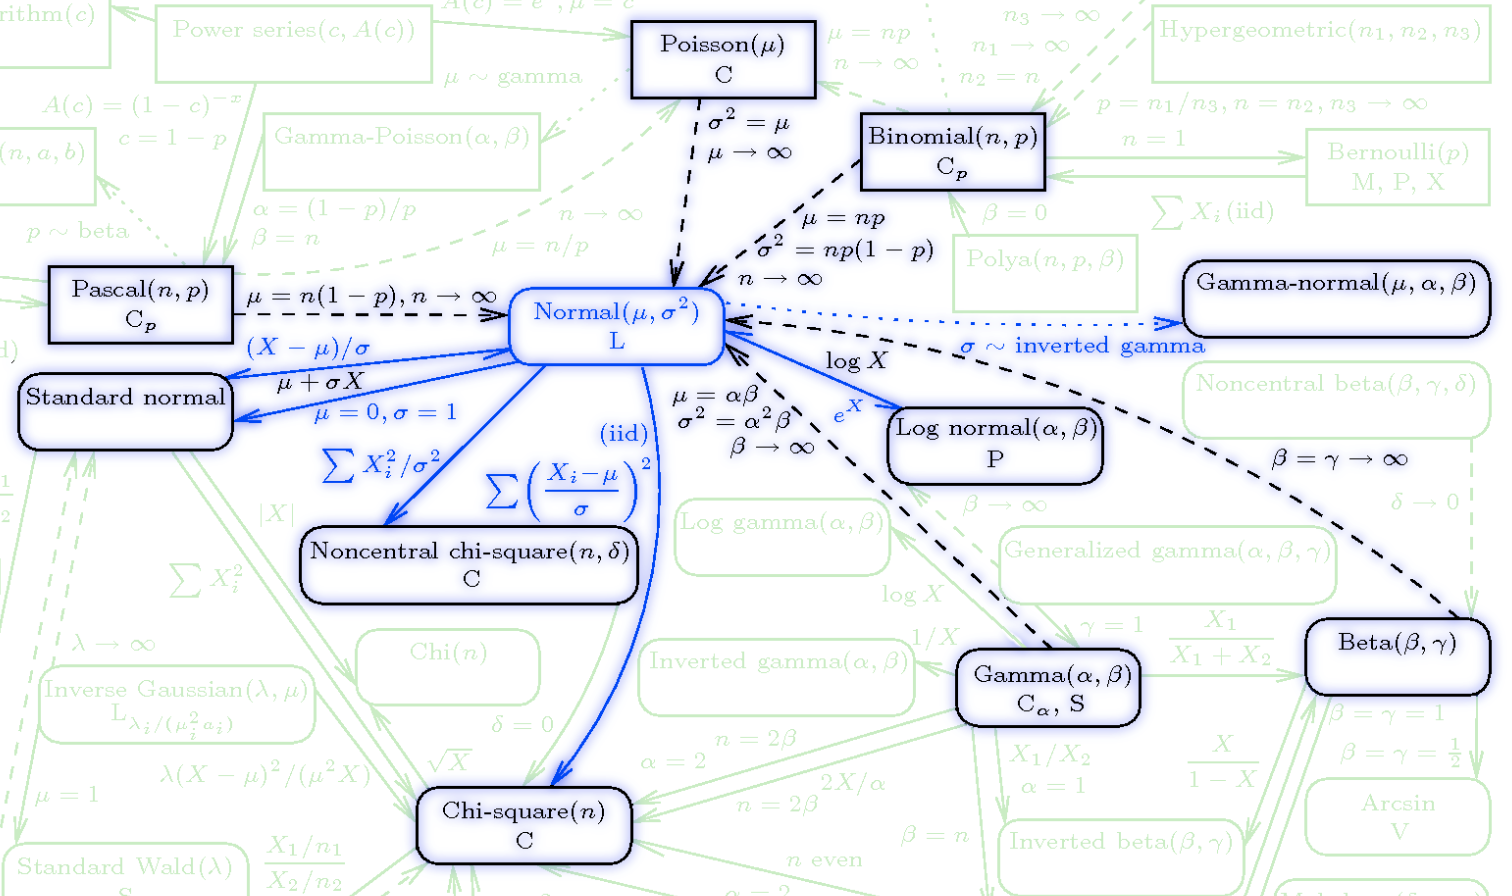
\includegraphics[height=10cm]{UDR.png}
\caption{\tiny{A snapshot of the UDR shows how the normal distribution can be transformed into a multitude of other distributions.}}
\end{figure}

\tiny{Hakaru functions representing probabilistic models (i.e. functions with a {\tt \tiny{measure(<type>)}} return type) cannot be used as operands in normal mathematical operations. This is to say we cannot transform models directly (i.e. we can’t do algebraic transformation on the PDF). The only operator we can use on a model is bind ({\tt \tiny{<$\sim$}}), to pull a sample from it. However, we are able to transform samples however we like. Therefore, we are interested in implementing transformations of the following form.}

\begin{equation*}
\begin{aligned}
& \tcboxmath[boxrule=2pt,colframe=MacMaroon]{R(p, q) \Rightarrow \textit{X} \sim A(p) \Rightarrow \textit{f(X)} \sim B(q)}
\end{aligned}
\end{equation*}

\bigskip

\tiny{In the equation above, \textit{p} is a set of values parameterizing the distribution \textit{A}}, \textit{q} is a set of values parameterizing the distribution \textit{B}, \textit{R(p, q)} is a set of relationships between \textit{p} and \textit{q} that must be satisfied, and \textit{f} is a function that applies a transformation to a sample. We can expand this definition to include transformations defined in terms of an aggregation of multiple independent samples. For example, the standard chi-square distribution is defined as the sum of the squares of \textit{n} normal random variables (see Figure 3). 

\begin{figure}
\centering
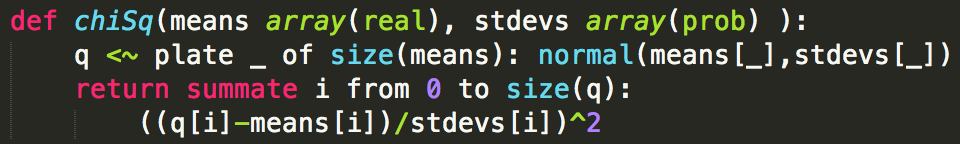
\includegraphics[height=3cm]{chi-square.png}
\caption{\tiny{Our implementation of the chi-square distribution.}}
\end{figure}

\bigskip



\end{block}

\end{textblock}

\end{textblock}


\begin{textblock}{5}(10.75,4)

\begin{variableblock}{}{}{}
\justifying

\tiny{Hakaru also lends itself very well to Bayesian transformations where we want to pull a sample from a distribution which is parameterized with a value sampled from another distribution. These transformations take the following form. Here, we are saying that if \textit{X} is parameterized by \textit{p}, then the distribution \textit{C}, which is parameterized by \textit{p} and \textit{q}, is equal to another distribution, \textit{B}, which is parameterized by \textit{q} and \textit{X}. The gamma-poisson distribution can be described by such a transformation (see Figure 4).}

\begin{equation*}
\begin{aligned}
& \tcboxmath[boxrule=2pt,colframe=MacMaroon]{X \sim A(p) \Rightarrow Y \sim B(q, X) = C(p, q)}
\end{aligned}
\end{equation*}

\begin{figure}
\centering
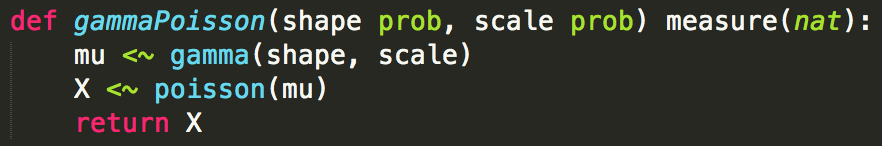
\includegraphics[height=3cm]{gamma-poisson.png}
\caption{\tiny{Our implementation of the gamma-poisson distribution.}}
\end{figure}

\bigskip

Some distributions on the UDR are unreachable from Hakaru's primitive distributions using transformations like the 2 described above. In these cases, we have to implement the model in terms of the PMF for a discrete distribution or in terms of the PDF for a continuous distributions. 


\end{variableblock}

%%%%%%%%%%%%%%%%%%%%%%%%%%%%%%%%%%%%%%%%%%%%%%%%%%%%%%%%%%%%%%%%%%%%%%
% Testing Relationships Between Distributions
%%%%%%%%%%%%%%%%%%%%%%%%%%%%%%%%%%%%%%%%%%%%%%%%%%%%%%%%%%%%%%%%%%%%%%

\begin{block}{Testing Relationships Between Distributions}
\justifying

\tiny{Recall that when developing the standard library, the UDR chart often implied multiple possible implementations for a given distribution. Naturally, we would expect alternative implementations for the same distribution to result in equivalent probabilistic models. This line of thought is the basis for the kinds of test cases we have implemented. More generally, we have the following hypothesis.}

\bigskip

\tiny{Assume we know a proven relationship between 2 statistical distributions, A and B, which allows us to transform A and B into distributions that are equivalent to each other. Further assume this transformation takes on one of the forms discussed in the Standard Library Development section. We hypothesize that by applying the appropriate transformations to implementations of A and B, we can create two Hakaru programs whose `hk-maple' outputs will be equivalent to each other. Test cases that prove our hypothesis true indicate the validity of the Hakaru language implementation. Test cases that prove our hypothesis false indicate an underlying bug in the language definition which is to be passed back to the language developers.
}

\end{block}

%%%%%%%%%%%%%%%%%%%%%%%%%%%%%%%%%%%%%%%%%%%%%%%%%%%%%%%%%%%%%%%%%%%%%%
% Conclusions & Future Work
%%%%%%%%%%%%%%%%%%%%%%%%%%%%%%%%%%%%%%%%%%%%%%%%%%%%%%%%%%%%%%%%%%%%%%

\begin{block}{Conclusions \& Future Work}

Conclusions \& Future Work

\end{block}

%%%%%%%%%%%%%%%%%%%%%%%%%%%%%%%%%%%%%%%%%%%%%%%%%%%%%%%%%%%%%%%%%%%%%%
% References
%%%%%%%%%%%%%%%%%%%%%%%%%%%%%%%%%%%%%%%%%%%%%%%%%%%%%%%%%%%%%%%%%%%%%%

\begin{block}{References}

References

\end{block}


% \begin{block}{References}
% \setbeamertemplate{bibliography item}{\insertbiblabel}
% \bibliographystyle{ieeetr}
% {\scriptsize
% \bibliography{../bib}}
% \end{block}

\end{textblock}
\end{frame}
\end{document}
